% STATUS: SSOT -- taylor gain (dual-machine rule 6)
% ======================================================
% Compile: xelatex 4state_taylor_gain.tex
% Path:    reference/eq17_analysis/derivation/4state_taylor_gain.tex
% Complete standalone derivation of the taylor-gain 4-state eq17 model:
% the gain state as a first-order Taylor expansion of a_x about the DESIRED
% trajectory, with the slope a'_x supplied exogenously. Replaces the RW /
% AR(1) surrogate stories: predict, F_e row 4, and the rank-1 Q block are
% all derived, not chosen. Includes the a' acquisition, the implemented
% feedforward forms, the R22 delay-term factor, and verification figures.
% Base chain (control law, eps, output equations): 4state_del_hd.tex.
% Code SSOT: model/controller/motion_control_law_eq17_4state.m
%            (knobs use_taylor_gain / aprime_source, default off),
%            model/controller/build_eq17_6state_constants.m.
% Style mirrors 4state_del_hd (monochrome, \fbox on key results, terse).
% ======================================================
% fontset=none: no CJK text; compiles anywhere.
\documentclass[11pt,a4paper,fontset=none]{ctexart}

\usepackage[fleqn]{amsmath}
\usepackage{amssymb,bm}
\usepackage{empheq}
\setlength{\mathindent}{0pt}
\usepackage{geometry}
\geometry{margin=2.0cm}
\usepackage{enumitem}
\usepackage{graphicx}

\setlength{\parindent}{0pt}
\setlength{\parskip}{0.3em}
\setlength{\abovedisplayskip}{4pt}
\setlength{\belowdisplayskip}{4pt}
\setlength{\abovedisplayshortskip}{2pt}
\setlength{\belowdisplayshortskip}{2pt}

\newcommand{\lc}{\lambda_c}
\newcommand{\hd}[1]{\par\medskip\noindent\underline{\textbf{#1}}\par\nobreak\vspace{0.2ex}}

\begin{document}

\hd{Equation of motion}
\[ x[k+1] = x[k] + a_x[k]\{f_{dx}[k] + f_T[k]\} + \delta x_D[k],
\qquad a_x = \Delta t/\gamma(h) \]

\hd{Measurement} (\textit{d}-step delay)
\[ \delta x_m[k] = \delta x[k-d] + n_x[k], \qquad \delta x = x_d - x \]

\hd{Control effort}
\begin{empheq}[box=\fbox]{equation*}
f_{dx}[k] = \hat a_x^{-1}[k]\Big\{ \Delta x_d^{d}[k]
+ (1-\lc)\Big[\delta x_m[k] - \textstyle\sum_{i=1}^{d}\hat a_x[k-i]\, f_{dx}[k-i]\Big] \Big\}
\end{empheq}

\hd{Motion error}
\begin{empheq}[box=\fbox]{equation*}
\delta x[k+1] = \lc\,\delta x[k] - F_{dx}[k]\, e_{a_x}[k]
- \underbrace{\Big\{ \delta x_T^{d}[k] - \delta x_{\delta a f}^{d}[k] + (1-\lc)\, n_x[k] \Big\}}_{\varepsilon[k]}
\end{empheq}
\[
F_{dx}[k] = f_{dx}[k] + (1-\lc)\sum_{i=1}^{d} f_{dx}[k-i],
\qquad e_{a_x} = a_x - \hat a_x,
\qquad \sigma^2_{\delta h} := 4 k_B T\, a_x
\]
\[
\sigma^2_\varepsilon := \gamma_\varepsilon(0) = \big(1 + 2(1-\lc)^2\big)\,\sigma^2_{\delta h} \;(= Q_{33});
\qquad
\text{AR(1) white driver: } (3-2\lc^2)\,\sigma^2_{\delta h};
\qquad
\tfrac{3-2\lc^2}{1+2(1-\lc)^2} = 1.712 \;(\lc{=}0.7)
\]

\hd{Gain model (first-order Taylor about the desired trajectory)}
\[ x[k+1] = x_d[k+1] - \delta x[k+1] \]
\[
a_x[k+1] = a_x\big(x[k+1]\big)
= \underbrace{a_x\big(x_d[k+1]\big)}_{a_{x_{det}}[k+1]} - \; a'_x[k+1]\,\delta x[k+1]
\]
\[
a_{x_{det}}[k+1] = a_{x_{det}}[k] + a'_x[k]\,\Delta h_d[k],
\qquad \Delta h_d[k] = h_d[k+1] - h_d[k],
\qquad a'_x[k+1] \approx a'_x[k] =: a'_x
\]

\hd{True recursion} \; ($a_{x_{det}}[k] = a_x[k] + a'_x\,\delta x[k]$, then the boxed $\delta x$ recursion)
\begin{empheq}[box=\fbox]{equation*}
a_x[k+1] = a_x[k] + a'_x\,\Delta h_d[k]
+ (1-\lc)\,a'_x\,\delta x[k]
+ a'_x\, F_{dx}[k]\, e_{a_x}[k]
+ a'_x\,\varepsilon[k]
\end{empheq}

\hd{Estimator (predict + update)} \; ($E\{e_{a_x}\}=0$, $E\{\varepsilon\}=0$; $\delta x[k] \to \delta\hat x_3[k]$)
\begin{empheq}[box=\fbox]{equation*}
\hat a_x[k+1] = \hat a_x[k] + a'_x\,\Delta h_d[k] + (1-\lc)\,a'_x\,\delta \hat x_3[k]
+ \ell_{41}[k]\, e_{y_1}[k] + \ell_{42}[k]\, e_{y_2}[k]
\end{empheq}

\hd{Error dynamics} \; ($e_{\delta x_3} = \delta x_3 - \delta\hat x_3$)
\begin{empheq}[box=\fbox]{equation*}
e_{a_x}[k+1] = \big(1 + a'_x F_{dx}[k]\big)\, e_{a_x}[k]
+ (1-\lc)\,a'_x\, e_{\delta x_3}[k]
+ \underbrace{a'_x\,\varepsilon[k]}_{q_4[k]}
- \ell_{41}[k]\, e_{y_1}[k] - \ell_{42}[k]\, e_{y_2}[k]
\end{empheq}

\hd{$\mathbf{F}_e$}
\begin{empheq}[box=\fbox]{equation*}
\mathbf{F}_e[k] =
\begin{bmatrix}
0 & 1 & 0 & 0 \\
0 & 0 & 1 & 0 \\
0 & 0 & \lc & -F_{dx}[k] \\
0 & 0 & (1-\lc)\,a'_x & \;1 + a'_x F_{dx}[k]
\end{bmatrix},
\qquad
\mathrm{eig}(\mathbf{F}_e) = \{\,0,\;0,\;\lc + a'_x F_{dx},\;1\,\}
\end{empheq}

\hd{Process noise (rank-1)} \; ($q_3 = -\varepsilon$, $q_4 = a'_x\,\varepsilon$: one sample)
\[
\mathbf{q}[k] = \varepsilon[k]
\begin{bmatrix} 0 \\ 0 \\ -1 \\ a'_x \end{bmatrix}
\quad\Rightarrow\quad
\mathbf{Q}[k] = \sigma^2_\varepsilon
\begin{bmatrix} 0 \\ 0 \\ -1 \\ a'_x \end{bmatrix}
\begin{bmatrix} 0 \\ 0 \\ -1 \\ a'_x \end{bmatrix}^{\!\top}
\]
\begin{empheq}[box=\fbox]{equation*}
Q_{33} = \sigma^2_\varepsilon,
\qquad
Q_{34} = Q_{43} = -\,a'_x\,\sigma^2_\varepsilon,
\qquad
Q_{44} = a'^2_x\,\sigma^2_\varepsilon
\end{empheq}
\[
P_{44} = a'^2_x\,P_{33},\qquad P_{34} = -a'_x\,P_{33}
\qquad (\text{exact filter invariant, } \forall R_{22})
\]
\[
\tfrac{\gamma_\varepsilon(0)}{1-\lc^2} = 2.31\,\sigma^2_{\delta h}
\;\;\text{vs}\;\;
\mathrm{Var}(\delta x) = C_{\delta x}\,\sigma^2_{\delta h} = 3.96\,\sigma^2_{\delta h},
\qquad C_{\delta x} = 2 + \tfrac{1}{1-\lc^2}
\quad (\varepsilon \text{ is MA}(d)\text{, not white})
\]

\hd{Feedforward (implemented forms)}
\[
\text{known: } \Delta\hat a = a_{x_{det}}[k] - a_{x_{det}}[k-1];
\qquad
\text{ahat: } \Delta\hat a = \hat a_x\Big(\tfrac{a_{x_{det}}[k]}{a_{x_{det}}[k-1]} - 1\Big);
\qquad
\text{diff: } \Delta\hat a = \hat a'_x\,\Delta h_d[k-1]
\]

\hd{$a'_x$ acquisition}
\[
\text{known: } a'_x = -\tfrac{a_{x_{det}}(\bar h_d)\,K_h(\bar h_d)}{R};
\qquad
\text{ahat: } a'_x = -\tfrac{\hat a_x[k]\,K_h(\bar h_d)}{R};
\qquad K_h = \tfrac{1}{c}\tfrac{dc}{d\bar h}
\]
\[
\text{diff: }\;
a'_{raw}[k] = \frac{\hat a_x[k] - \hat a_x[k-1]}{\Delta h_d[k-1]},
\qquad \text{update iff } \big|\Delta h_d[k-1]\big| \ge \gamma
\]
\begin{empheq}[box=\fbox]{equation*}
\hat a'_x[k] = (1-\beta)\,\hat a'_x[k-1] + \beta\, a'_{raw}[k],
\qquad \beta = 0.05,\quad \gamma = 10^{-3}\,\mu\mathrm{m};
\qquad \hat a'_x \leftarrow \max(\hat a'_x, 0)\ \text{(optional)}
\end{empheq}

\hd{$R_{22}$ delay term} \; ($r_2 = n_a - \sum_{i=1}^{d}\Delta a_{ram}[k-i]$, $d=2$)
\[
\Delta a_{ram}[k-1] + \Delta a_{ram}[k-2] = a_{ram}[k] - a_{ram}[k-2]
\;\Rightarrow\;
\mathrm{Var}\Big(\textstyle\sum\Big) = 2\,(1-\rho_2)\,\mathrm{Var}(a_{ram})
\]
\begin{empheq}[box=\fbox]{equation*}
R_{22}^{delay} = \frac{1-\rho_2}{2\,(1-\rho_1)}
\sum_{i=1}^{d} \mathrm{Var}\big(\Delta a_{ram}[k-i]\big),
\qquad
\frac{1-\rho_2}{2(1-\rho_1)} = 1.105 \;(\lc{=}0.7)
\end{empheq}
\[
\rho_1 = 0.8515,\quad \rho_2 = 0.6718
\qquad (\rho_\tau = \text{lag-}\tau\ \text{autocorr of } \delta x)
\]

\newpage
\begin{center}
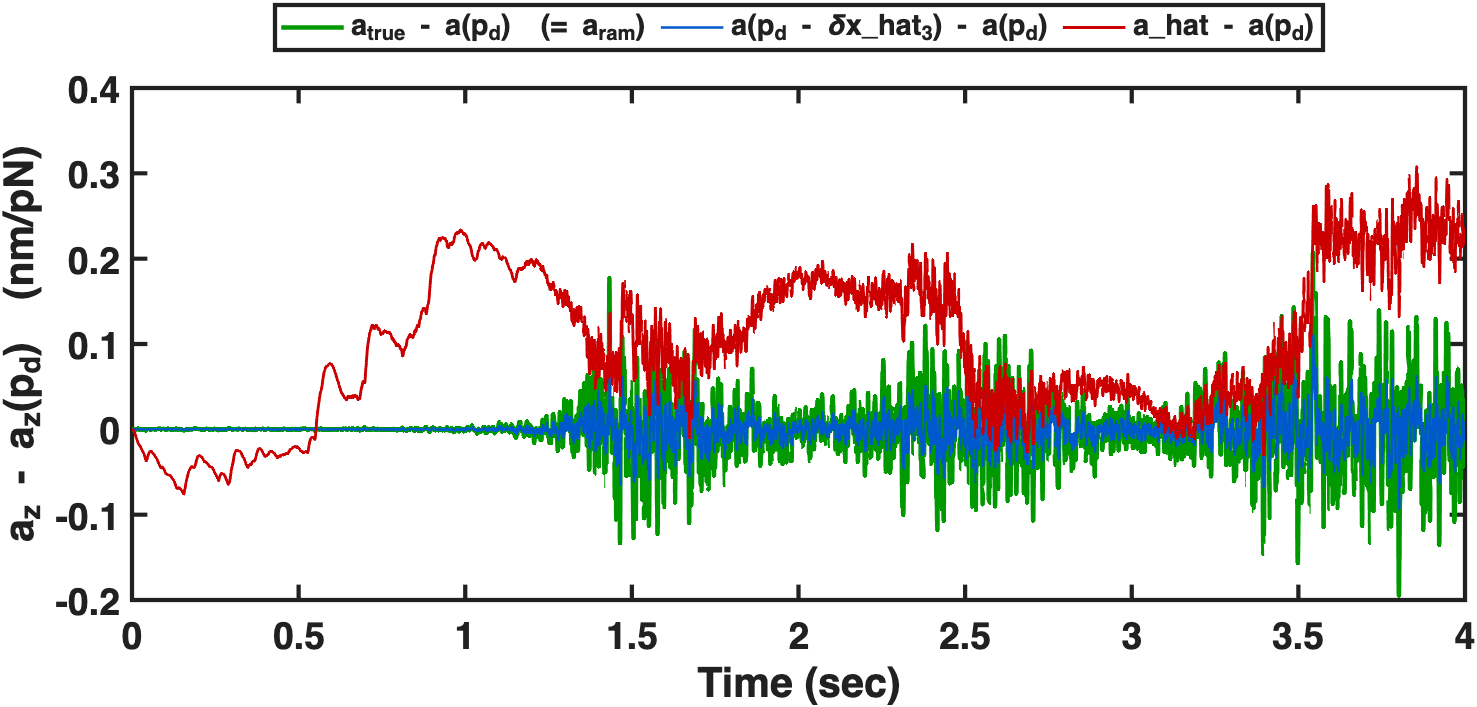
\includegraphics[width=0.92\textwidth]{figures/fig_taylor_gap_known_z.png}
\end{center}
Oracle-$a'$ arm, $z$ axis, 1 Hz osc, seed 1:
$\hat a_x - a_x(p_d)$ vs $a_{x,true} - a_x(p_d)$ ($= a_{x_{ram}}$).

\begin{center}
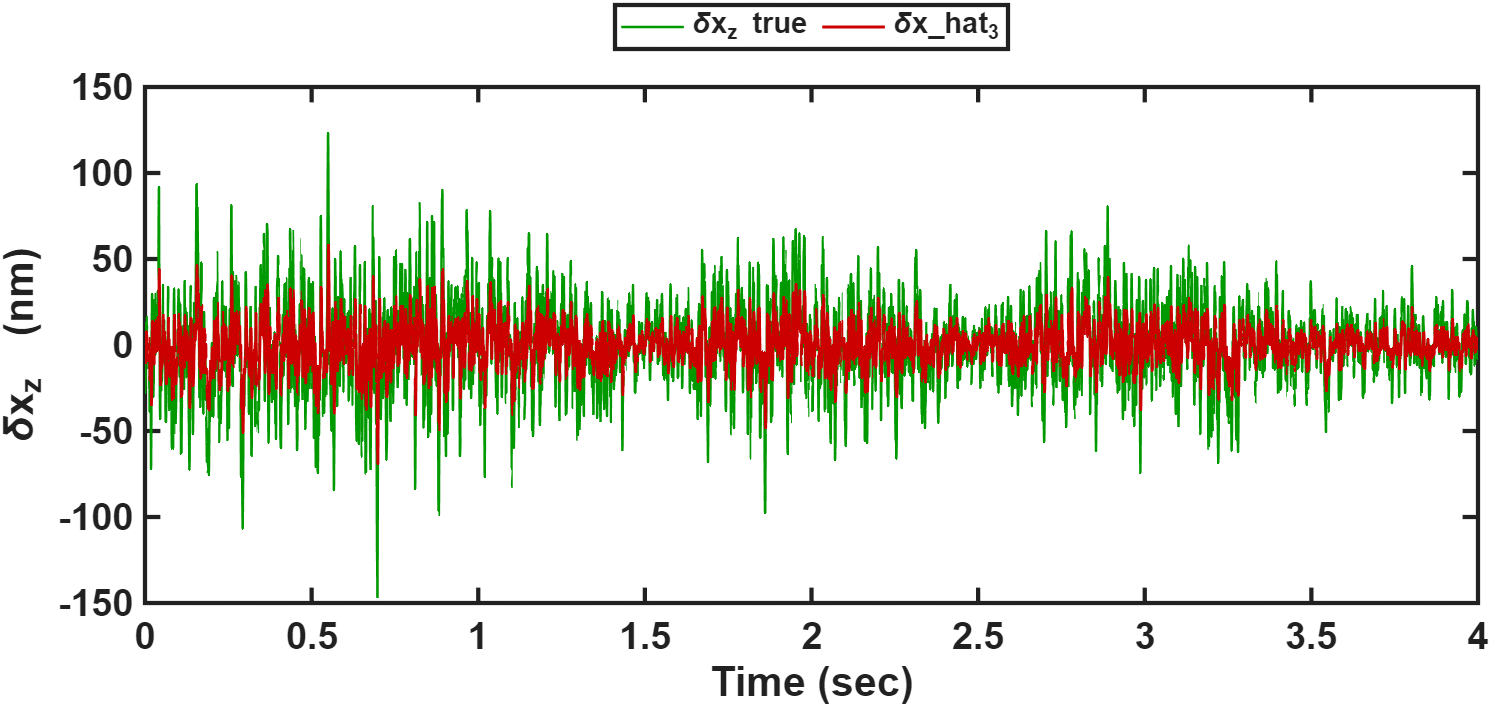
\includegraphics[width=0.92\textwidth]{figures/fig_taylor_dx3_known_z.png}
\end{center}
Same arm and seed: $\delta\hat x_3$ vs true $\delta x_z$.

\begin{center}
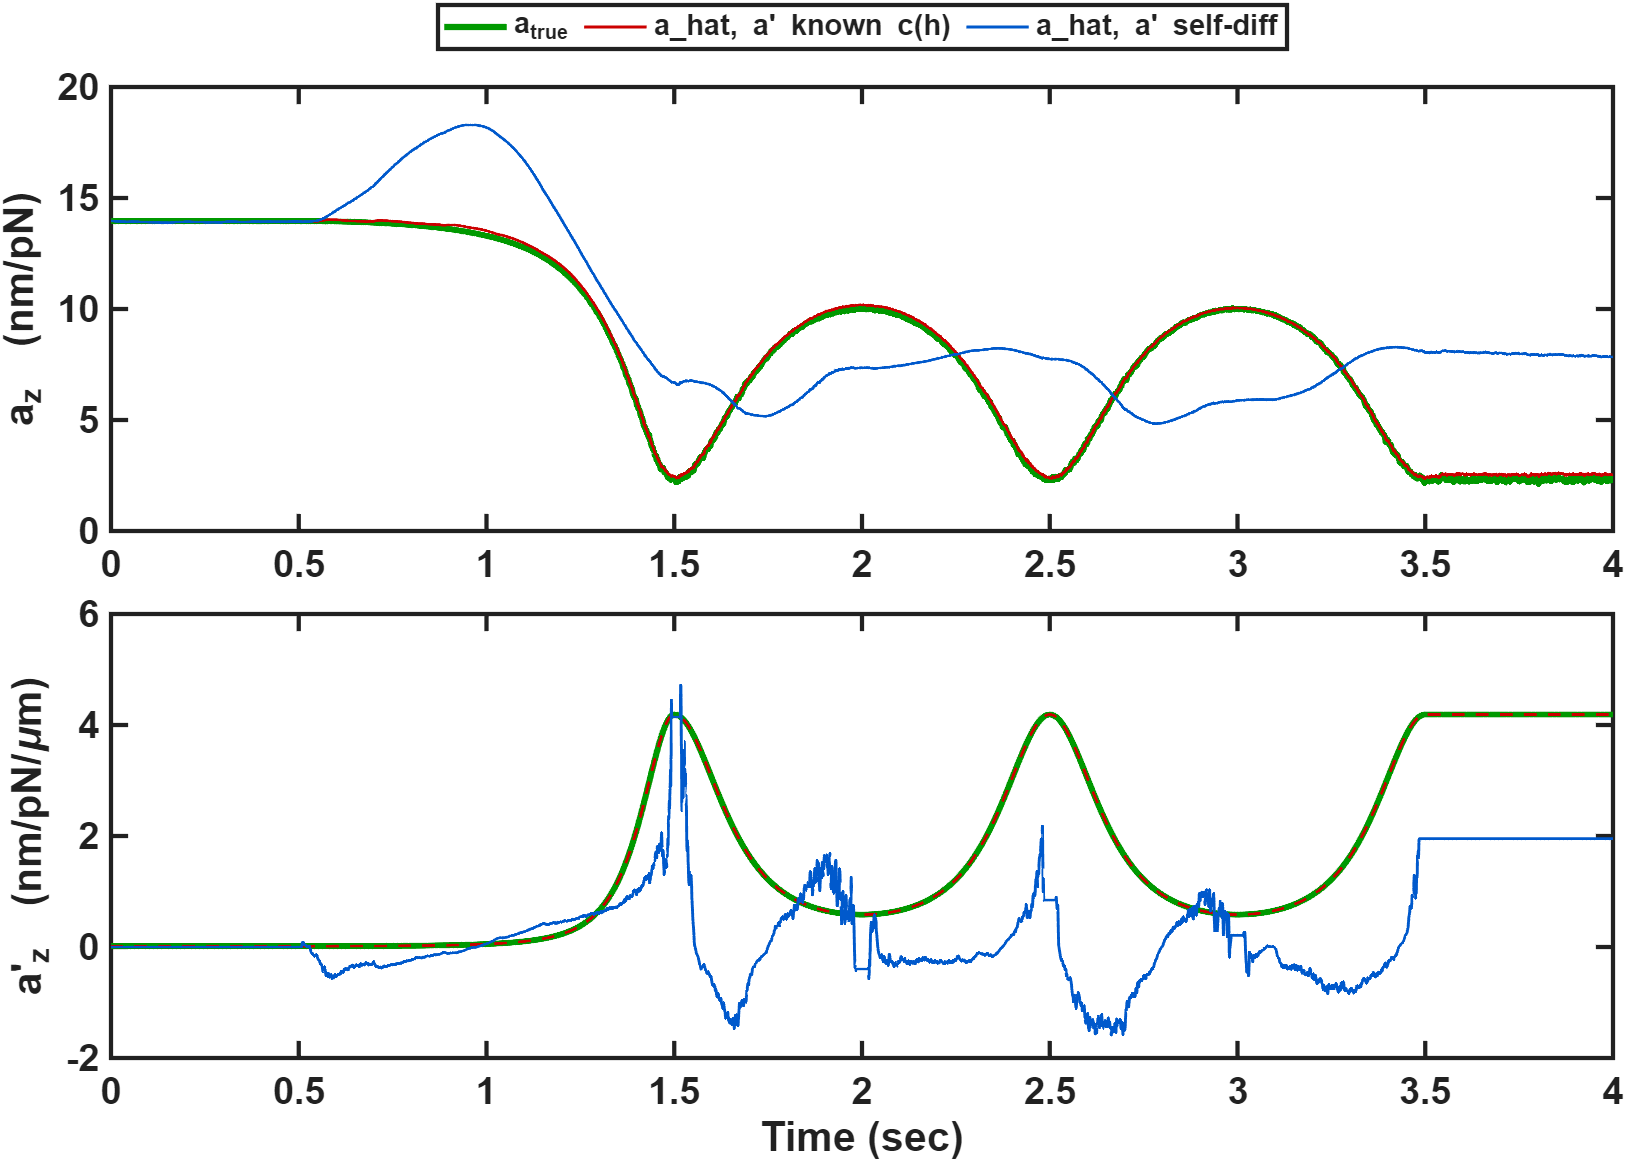
\includegraphics[width=0.92\textwidth]{figures/fig_taylor_overlay_stacked_z.png}
\end{center}
Same seed: $\hat a_x$ (top) and $a'_x$ (bottom), oracle-$a'$ arm vs self-diff arm (no clamp).

\begin{center}
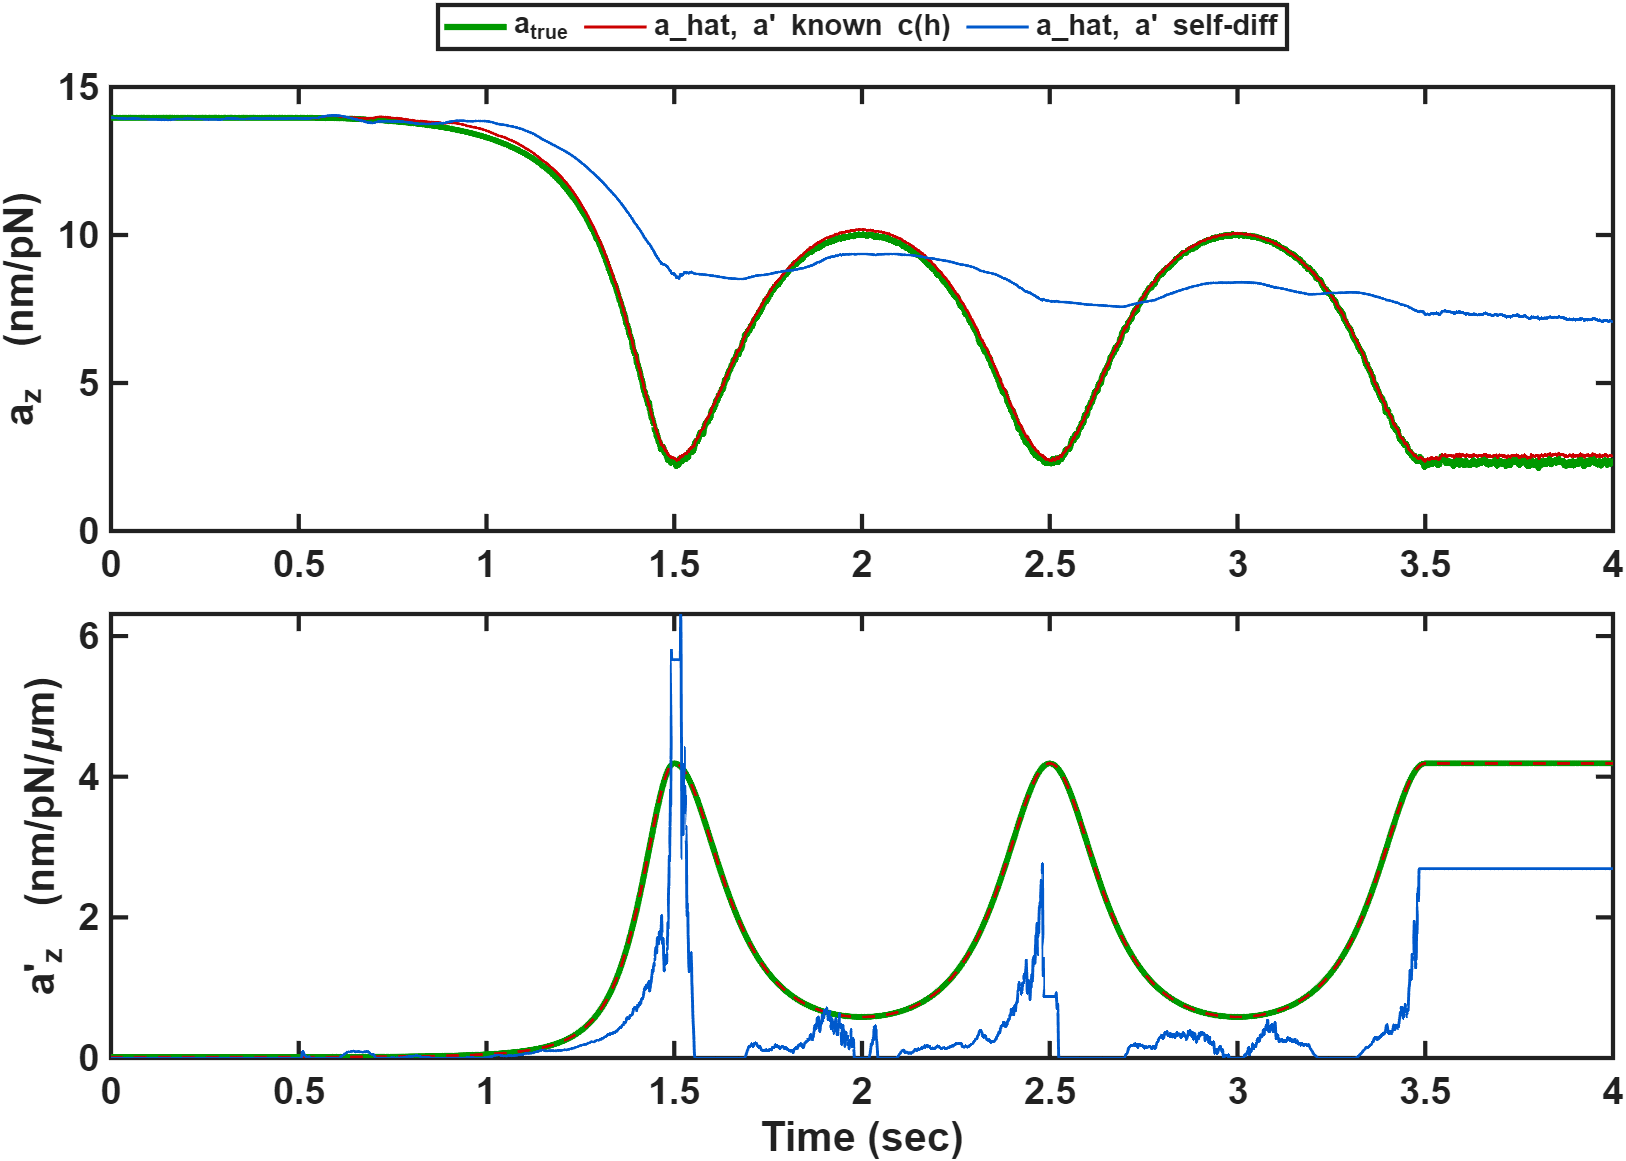
\includegraphics[width=0.92\textwidth]{figures/fig_taylor_overlay_stacked_z_clamp.png}
\end{center}
Same seed with the post-EWMA clamp $\hat a'_x \leftarrow \max(\hat a'_x, 0)$.

\end{document}
